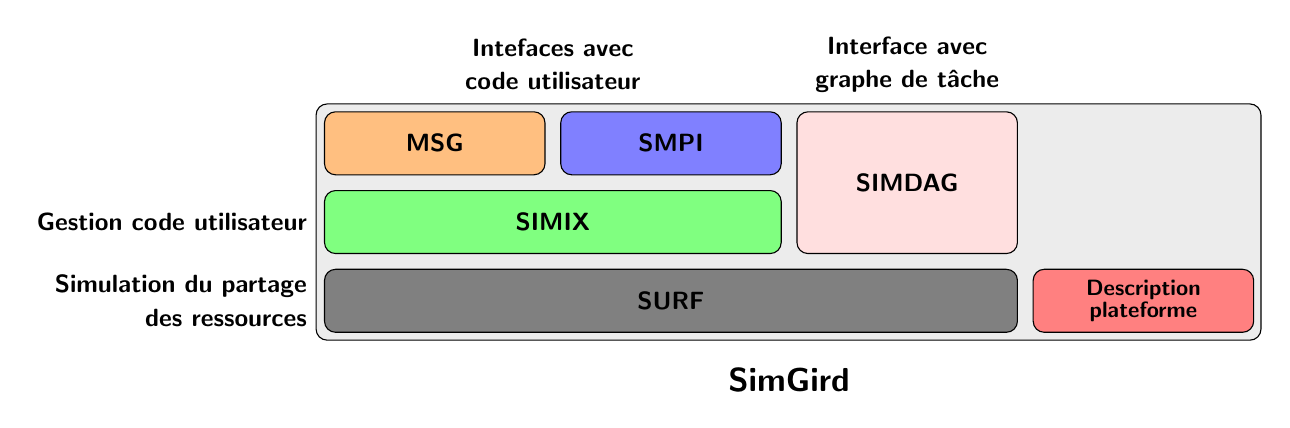
\begin{tikzpicture}[x=3cm,y=1cm,
base/.style={
rounded corners,
draw,
outer sep=1mm,
anchor=west,
},
black/.style={
font={\sffamily\bfseries\color{black} \fontsize{9pt}{12}\selectfont},
},
white/.style={
font={\sffamily\bfseries\color{white} \fontsize{9pt}{12}\selectfont},
},
elevel/.style={
align=right,
anchor=east
},
wlevel/.style={
align=left,
anchor=west
},
level/.style={
align=center,
},
w1/.style={
base,
minimum width=2.8cm,
minimum height=0.8cm,
},
w2/.style={
base,
minimum width=5.8cm,
minimum height=0.8cm,
},
w3/.style={
base,
minimum width=8.8cm,
minimum height=0.8cm,
},
h2/.style={
base,
minimum width=2.8cm,
minimum height=1.8cm,
},
bg/.style={
draw,
rounded corners,
fill=gray!15,
anchor=east,
},
]
\node[bg,minimum width=12cm,minimum height=3cm]at(4,1){};
\node[level,font={\sffamily\bfseries\color{black} \fontsize{12pt}{12}\selectfont}]at(2,-1){SimGird};
\node[level,black]at(1,3){Intefaces avec \\code utilisateur};
\node[w1,fill=orange!50,black]at(0,2){MSG};
\node[w1,fill=blue!50,black]at(1,2){SMPI};
\node[elevel,black]at(0,1){Gestion code utilisateur};
\node[w2,fill=green!50,black]at(0,1){SIMIX};
\node[level,black]at(2.5,3){Interface avec\\graphe de t\^ache};
\node[h2,fill=pink!50,black]at(2,1.5){SIMDAG};
\node[elevel,black]at(0,0){Simulation du partage\\des ressources};
\node[w3,black,fill=gray]at(0,0){SURF};
\node[w1,fill=red!50,align=center,font={\sffamily\bfseries\color{black} \fontsize{8pt}{0}\selectfont}]at(3,0){Description\\plateforme};

\end{tikzpicture}